\section{Genesis Network}

The Genesis Network is a special set of validators and full nodes that will be used during launch. Hosts of the genesis network will be geographically distributed across different AWS regions. These regions will be linked via VPC peering, so traffic inside the genesis network is not public facing. \\

The genesis network will be run by the EnergyWeb Foundation.

\begin{figure}[ht]
	\centering
    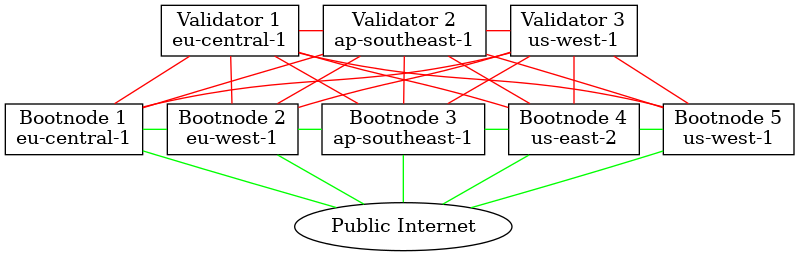
\includegraphics[width=0.85\textwidth,keepaspectratio]{./images/genesis-network.png}
	\caption{Genesis Network Layout}
	\label{fig:genesisnet}
\end{figure}

\subsection{Validators}

The genesis validators will be starting the chain and also their validator account addresses are hard coded as constructor arguments to the validator contract in the chain specification. The hosts running those validator nodes adhere to the same security standards as normal validators with the addition that they don't have any connection to the public internet blockchain wise. \\
The following outgoing traffic is permitted though an AWS NAT gateway:

\begin{itemize}
    \item DNS (53/UDP+TCP)
    \item HTTP (80/TCP) - mainly for sys updates
    \item HTTPS (443/TCP) - mainly for sending telemetry
\end{itemize}

Blockchain traffic is only allowed inside the AWS VPC to the Bootnodes. The validators will have a special configuration file for parity to facilitate that along with the following security group settings

\begin{itemize}
    \item Allow P2P traffic (30303/tcp+udp) inbound only from the bootnodes via RFC1918 inside the VPC
    \item Allow P2P traffic (30303/tcp+udp) outbound only to the bootnodes via RFC1918 inside the VPC
    \item Allow SSH traffic only inbound via a jump host inside the VPC over RFC1918
\end{itemize}

A preferred EC2 Instance type would be c5.xlarge. These nodes also don't have dedicated public IP's

\subsection{Bootnodes}

The genesis bootnodes are regular fullnodes (state pruned, no tracing, no fatdb, no warp).
They accept connections from the public internet and the validator VPC's on their blockchain P2P port.

Enode addresses of those bootnodes will be part of the general public chainspec.

